\documentclass[../main/main.tex]{subfiles}
\begin{document}

%\dominitoc
%\faketableofcontents
\setcounter{chapter}{5}
\chapter{Modélisation hyperspectrale}\label{ch:modelhyperspec}

\minitoc
\vspace{2cm}
Ce chapitre est consacré l'étape de construction du cube intrinsèque de
la galaxie hôte, que nous avons introduit dans le
chapitre~\ref{ch:hypergal}.

Nous présenterons dans un premier temps le relevé Pan-STARRS, les images photométriques
qui serviront de base d'information pour notre modélisation hyperspectrale et les
étapes de pré-traitement à appliquer.

Puis nous introduirons le SED Fitter \pkg{CIGALE}, qui sera utilisé pour
obtenir une SED de la galaxie à l'échelle locale, la configuration
implémentée et son application aux images photométriques.

Enfin, nous détaillerons la construction du cube intrinsèque, étape
finale de la modélisation hyperspectrale de la galaxie.
\newpage

\section{Source photométrique}
\label{sec:photosource}

Notre cadre de recherche étant au sein de la collaboration ZTF, nous
devons prévoir le fait que nous aurons des alertes d'évènements
transitoires dans tout le ciel Nord, couverture du sondage. Par
ailleurs, le but d'\hypergal\ étant une modélisation de scène d'une
observation de la SEDm, la source photométrique utilisée doit avoir a
minima la même profondeur en magnitude. Enfin, la projection se faisant
de l'espace photométrique vers l'espace des observables de la SEDm, il
serait plus judicieux d'utiliser un relevé photométrique attestant d'un
meilleur seeing, pour éviter de dégrader les données.

Le relevé Pan-STARRS1 du système Pan-STARRS - \textit{Panoramic Survey Telescope and Rapid
Response System} - \citep{Kaiser2002,Kaiser2010} répond à tous ces critères. C'est d'ailleurs basée sur
la première Data Release de ce relevé astronomique \citep{ChambersPanstarrs,Flewelling2020} que la procédure de calibration photométrique
de ZTF est effectuée.

\subsection{Relevé astronomique Pan-STARRS1}
\label{ssec:ps1}

Le relevé Pan-STARRS1 \citep{ChambersPS1survey} est une installation innovante d’imagerie
astronomique à grand champ,
développé à l'Institut d'astronomie de l'Université de Hawaï. Le relevé
Pan-STARRS1 vient du nom du premier télescope du projet situé à l'Observatoire Haleakala,
Pan-STARRS Telescope \#1 ou encore PS1. L'optique de PS1 est décrit dans
\citet{Hodapp2004a, Hodapp2004b, Hodapp2004c, Morgan2008}.
Ce télescope possède un miroir
primaire de \SI{1.80}{\meter} de diamètre avec une focale de \SI{8}{\meter}, et un miroir
secondaire de \SI{0.9}{\meter}. 

La caméra montée sur le télescope PS1 est la Gigapixel Camera \#1
(GPC1) de $1.4$ gigapixel, conçue au laboratoire Lincoln
\citep{Tonry2006GPC1,Tonry2008GPC1} et offrant un champ de vue d'environ
$3.3\degree$ de diamètre. 
Le plan focal de la caméra GPC1 est divisé en 60 structures OTA CCID58
(Orthogonal Transfer Array; \citet{Tonry1997OTA,Tonry2008GPC1}), où
chacun est composé d'un réseau de 8$\times$8 CCDs (cellules). Un unique
OTA est composé de 64 cellules de 590$\times$598 pixels de
$\SI{10}{\micro\metre}$ de côté. Une illustration du plan focal de la
caméra est présentée dans la Figure~\ref{fig:gpc1focalplan}.

\begin{figure}[h]
  \begin{minipage}[c]{0.4\textwidth}
    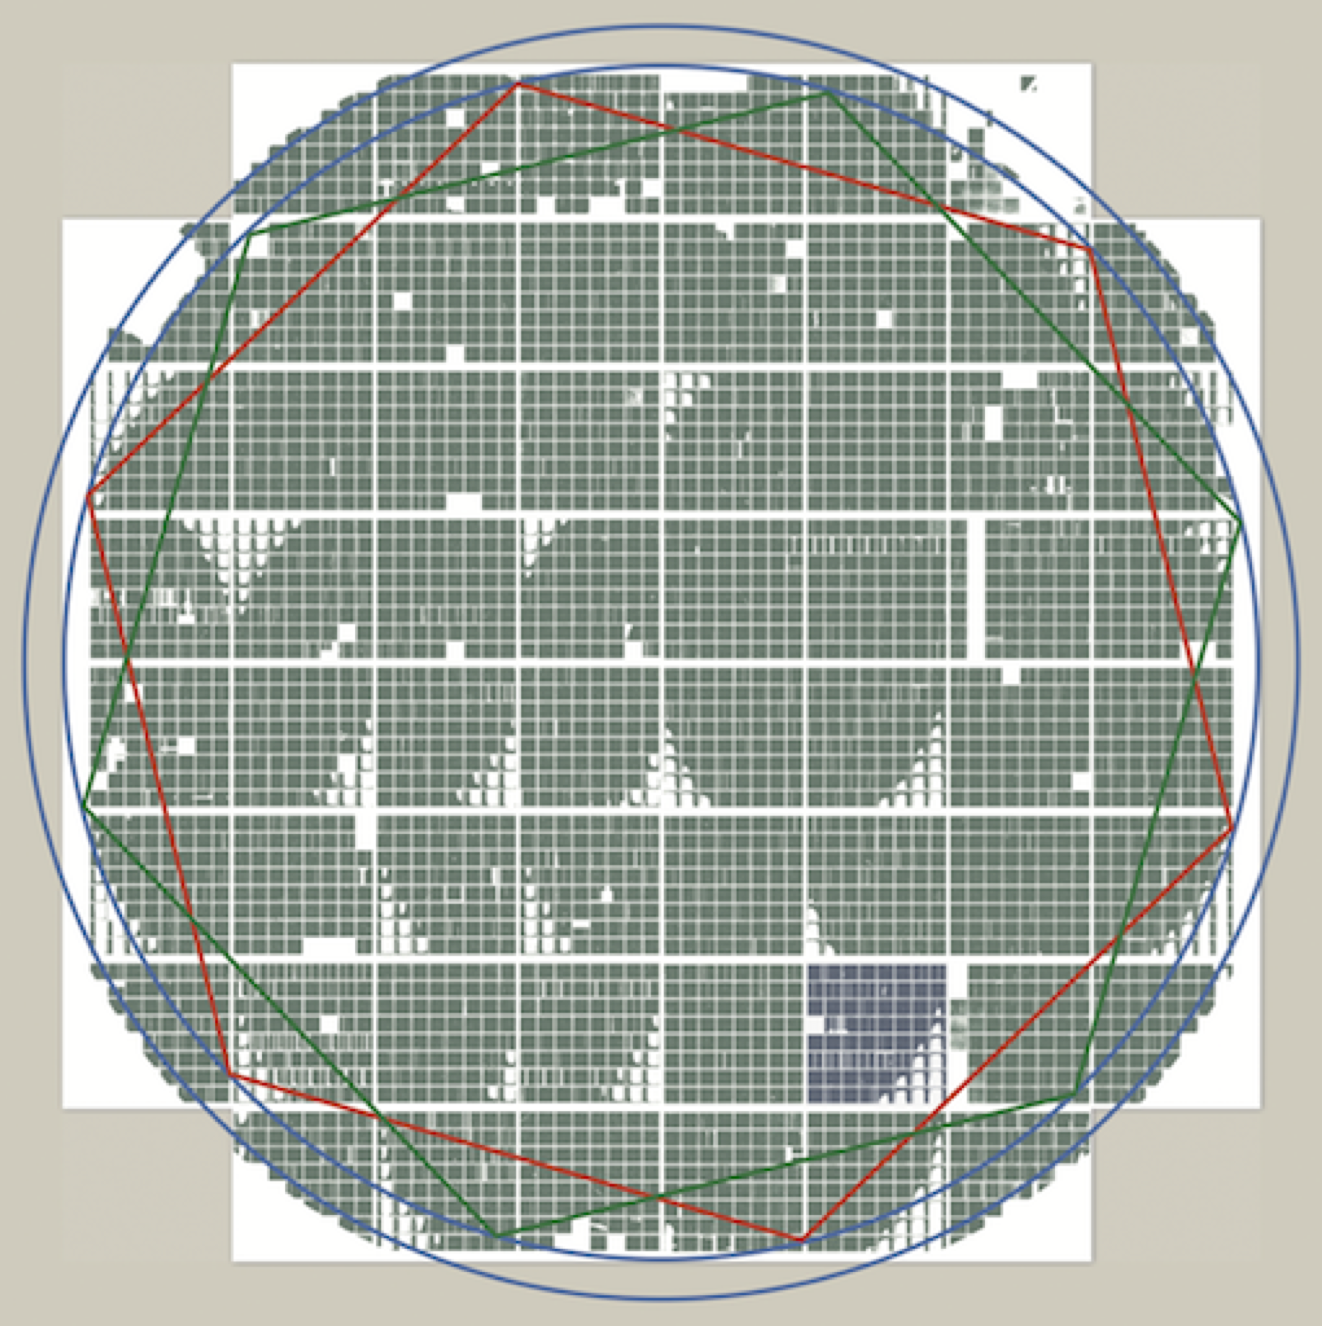
\includegraphics[width=\textwidth]{../figures/05_sedfit/GPC1focalplan.png}
  \end{minipage}\hfill
  \begin{minipage}[c]{0.5\textwidth}
    \caption[Plan focal de la Gigapixel Camera (PS1)]{Plan focal de la
    Gigapixel Camera (PS1) (figure de \citet{ChambersPS1survey}). Les cellules non fonctionnelles sont
    masquées et représentées en blanc dans la figure ci-dessus.}\label{fig:gpc1focalplan}
  \end{minipage}
\end{figure}


Une des missions de PS1 (à plus de $56\%$ du temps alloué) est l'observation de tout le ciel Nord à une déclinaison $\delta>30\degree$ :
c'est le
relevé $3\pi$ Stéradian. Les observations sont effectuées avec 5 filtres
$g_{P1}$, $r_{P1}$, $i_{P1}$, $z_{P1}$ et $y_{P1}$. On notera
l'existence d'un  sixième
filtre ($w_{P1}$) qui
englobe les filtres $g,r,i$ mais qui est utilisé pour l'étude du système
solaire et non le relevé $3\pi$ Stéradian. Les informations
de transmission de ces $6$ filtres sont présentées dans la Figure~\ref{fig:ps1filters}.

\begin{figure}
  \centering
  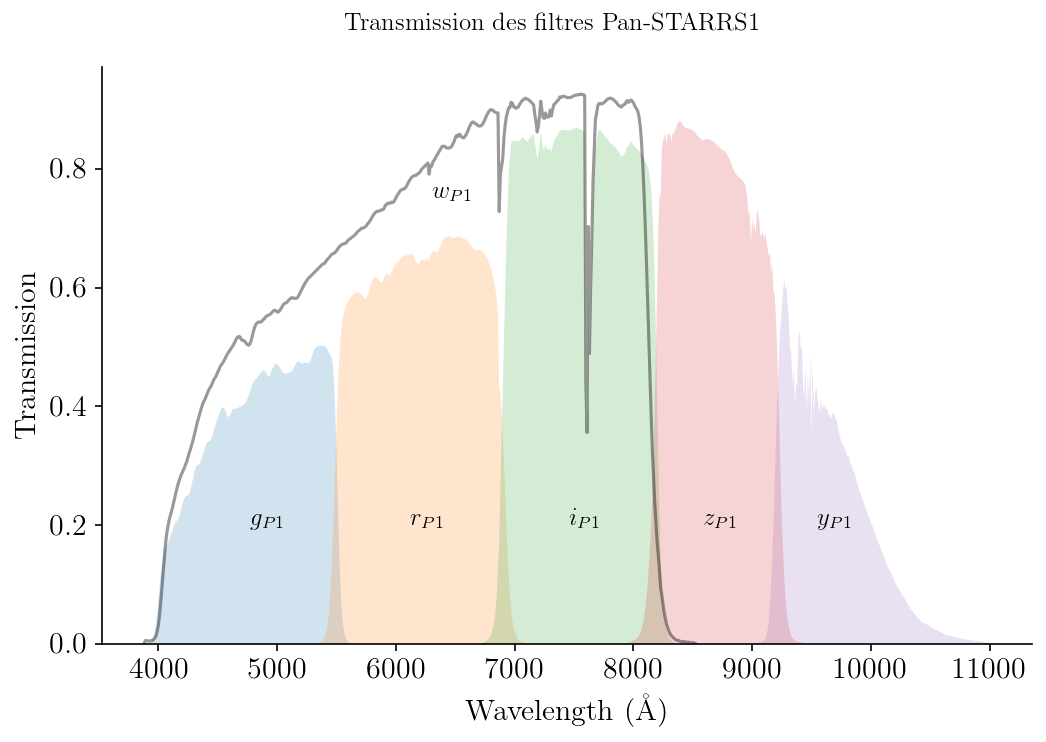
\includegraphics[width=0.8\textwidth]{../figures/05_sedfit/ps1filters.png}
  \caption[Transmission des filtres Pan-STARRS1]{Transmission des
    filtres $grizy$ de Pan-STARRS1 \citep{Tonry2012}.}
  \label{fig:ps1filters}
\end{figure}


Pan-STARRS1 utilise le système de magnitude ``AB'' \citep{Oke1983}
décrit en détail pour le relevé SDSS \citep{YorkSDSS2000} par
\citet{Fukugita1996}.

Dans ce système, une magnitude monochromatique AB est défini comme le
logarithme de la densité spectrale de flux, tel que:

\begin{align}
  \label{eq:abmag}
  m_{AB}(\nu)&= -2.5\log_{10}(f_{\nu}[\erg\ \text{s}^{-1}\cm^{-2}\Hz^{-1}]) -
  48.60\\
  m_{AB}(\nu)&= -2.5\log_{10}(\frac{f_{\nu}[\jy]}{3631\jy})
\end{align}
avec $1\text{Jy} = 10^{-23}\erg.\sec^{-1}\cm^{-2}\Hz^{-1}$.

La magnitude AB d'une bande passante est alors définie telle que:
\begin{equation}
  \label{eq:abmagbp}
  m_{AB}\approx-2.5\log_{10}\left(\frac{\int
      f_{\nu}(h\nu)^{-1}A(\nu)\d\nu}{\int 3631\jy(h\nu)^{-1}A(\nu)\d\nu}   \right)
\end{equation}
où $A(\nu)$ est la fonction de réponse du filtre considéré. Le système
photométrique de PS1 est détaillé dans \citet{Tonry2012}.

\begin{table}[h]
    \centerfloat
    \begin{threeparttable}
        \caption{Caractéristiques des filtres $grizy$ de PAN-STARRS1 et
          du relevé $3\pi$ Stéradian.}
        \label{tab:3pisteradian}
        \begin{tabular}{lccccccc}
            \toprule
             \multirow{2}[3]{*}{Filtres} & \multirow{2}[3]{*}{$\lambda_{pivot}$(\AA)} &                                                                    \multirow{2}[3]{*}{\# Expositions}  & \multirow{2}[3]{*}{\shortstack{mag
                                                  à $5\sigma$ \\(exposition unique)}} &
                                                                 \multirow{2}[3]{*}{\shortstack{mag
                                  à $5\sigma$ \\
          (expositions empilées)}} & \multirow{2}[3]{*}{\shortstack{Seeing
                                  \\médian ('') }} &  \multirow{2}[3]{*}{\shortstack{Mode
                                  \\seeing ('')}} \\
          \\
            & & & & & & \\
          \midrule
          $g_{P1}$ & $4849.11$ &60528 & $22.0$ & $23.3$ & $1.47$ & $1.31$\\
          $r_{P1}$ & $6201.20$ &70918 & $21.8$ & $23.2$ & $1.31$ & $1.15$\\
          $i_{P1}$ & $7534.96$ &104414& $21.5$ & $23.1$ & $1.19$ & $1.05$\\
          $z_{P1}$ & $8674.20$ &67604 & $20.9$ & $22.3$ & $1.14$ & $1.00$\\
          $y_{P1}$ & $9627.79$ &70982 & $19.7$ & $21.4$ & $1.09$ & $0.95$\\
                     
            \bottomrule
        \end{tabular}
        \begin{tablenotes}[flushleft]
        \item \textbf{Notes.} La longueur d'onde pivot $\lambda_{pivot}$
          est déterminée avec la transmission $A(\lambda)$ tel que
          $\lambda_{pivot}=\sqrt{\frac{\int A(\lambda)\d\lambda}{\int A(\lambda)\d\lambda/\lambda^{2}}}$.
        \end{tablenotes}
    \end{threeparttable}
\end{table}


Nous présentons dans la Table~\ref{tab:3pisteradian} quelques
caractéristiques des filtres $grizy$ de PS1, ainsi que du relevé $3\pi$
Stéradian.

\subsection{Utilisation des images PS1}
\label{ssec:preprocessps1}

Bien entendu nous n'utilisons pas les images brutes acquises par PS1,
mais celles ayant été traitées avec différentes étapes de corrections,
qui constituera in fine la $1\iere$ Data Release de PS1 \citep{ChambersPanstarrs,Flewelling2020}.
Ces étapes de traitement d'image sont détaillées dans
\citet{Waters2020}.

La section 3 de \citet{Waters2020} décrit la partie corrective des
images:

\begin{itemize}[label=$\diamondsuit$]
  \itemsep0em 
   \item \textbf{Soustraction du bias et du dark} pour prendre en compte
     le niveau de base(piédestal) de la caméra et le signal thermique en fonction du temps d'exposition.
   \item \textbf{Cartographie du bruit} (qui n'est pas forcément uniforme, mais peut
     présenter un gradient).
   \item \textbf{Division du flat} pour corriger les effets de vignettage. Les
     flats sont pris avec une exposition du ciel au
     crépuscule.
   \item  \textbf{Correction d'effets de franges} dans les images. Ces structures
     d'interférences sont notamment visibles vers l'infrarouge, où les
     longueurs d'ondes sont du même ordre de grandeur que l'épaisseur du
     détecteur.
   \item \textbf{Application d'un masque statique} pour les pixels du détecteur
     défectueux ou ayant une réponse très faible dans toutes les expositions, et un \textbf{masque dynamique}
     qui va varier pour chaque observation.
   \item \textbf{Correction d'effet de CTI} \textit{Charge Transfert Inefficiency}, dû à la saturation d'un
     pixel. Ce phénomène créé une trainée verticale partant du centre de
     la source de forte luminosité.
   \item \textbf{Correction des non-linéarités}, les pixels de la GPC1
     n'ayant pas une réponse strictement linéaire en fonction du niveau
     de flux. Ce phénomène est d'autant plus prononcé aux bords du
     détecteur et à bas flux.
   \item \textbf{Correction de motifs} notamment horizontaux dus à des
     effets de 
     diaphonies entre deux lignes de pixels adjacentes.
   \item \textbf{Modélisation et soustraction du fond du ciel}, une fois
     que toutes les corrections précédentes ont été appliquées.
\end{itemize}

L'étape suivante de traitement des images, décrite dans la section 5 de
\citet{Waters2020}, est une transformation géométrique des images
individuelles en un jeu d'image, créant une
relation cohérente et uniforme entre les pixels et les coordonnées du ciel. Cette transformation permet alors d'effectuer des opérations de
combinaison d'images superposants une partie commune du ciel. Dans ce
nouveau système d'agencement, les pixels ont alors une taille de
$0\farcs25$ de côté.


La section 6 de \citet{Waters2020} traite justement de la procédure
d'empilement d'images, permettant ainsi un meilleur rapport signal sur
bruit (SNR) dans les zones du ciel communes à plusieurs expositions. Cet
empilement est effectué de sorte que toutes les images aient un point
zero de $ZP=\SI{25.0}{mag}$, et une masse d'air de $z=1$. Ce
sont ces images traitées et empilées que nous utiliserons pour la
modélisation hyperspectrale des galaxies hôtes.


Nous utilisons pour cela le serveur libre d'accès aux images
PS1\footnote{\url{https://ps1images.stsci.edu/cgi-bin/ps1cutouts}},
permettant d'effectuer une requête d'images centrées sur une position du
ciel arbitraire (RA, DEC), et de côté arbitraire $N$ pixels, sachant que chaque pixel
est de forme carré de $0\farcs25$ de côté. Les images peuvent être
récupérées dans chacun des 5 filtres $g_{P1}$, $r_{P1}$, $i_{P1}$,
$z_{P1}$ et $y_{P1}$, avec un flux par pixel exprimé en unité de coups. Nous montrons dans la
Figure~\ref{fig:pscutoutsZTF18accrorf} une image de $140\times140$
pixels ($=35"\times35"$) centrée sur la position de détection par ZTF de
ZTF18accrorf. 

\begin{figure}[ht]
  \begin{minipage}[c]{0.45\textwidth}
    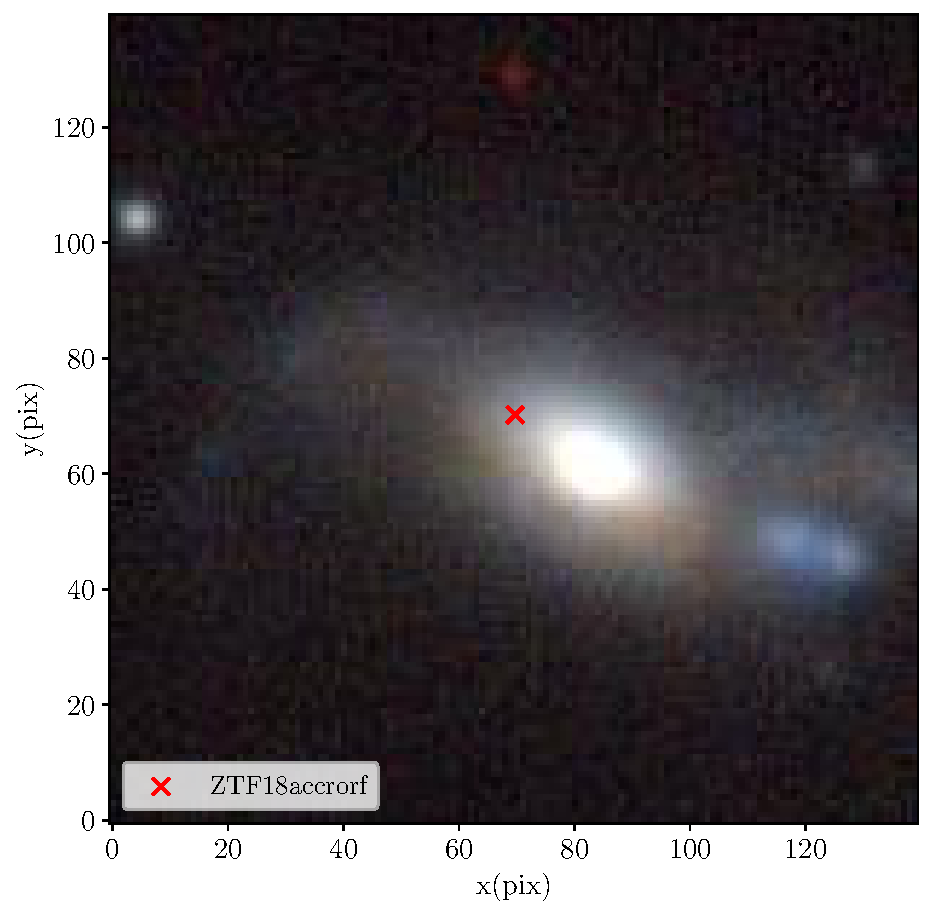
\includegraphics[width=\textwidth]{../figures/05_sedfit/ps_cutouts_ZTF18accrorf.pdf}
  \end{minipage}\hfill
  \begin{minipage}[c]{0.52\textwidth}
    \caption[Image RGB de PS1 centrée sur ZTF18accrorf.]{Image RGB
      construite à partir des bandes $g_{P1}$, $r_{P1}$ et
      $z_{P1}$ des images PS1. L'image fait $35"$ de côté et est centrée sur la position de
      détection de ZTF18accrorf par ZTF, à $(\text{RA}, \text{DEC})=(17.1692\degree,20.0799\degree)$}\label{fig:pscutoutsZTF18accrorf}
  \end{minipage}
\end{figure}


\section{\pkg{Cigale} et SEDFitting}
\label{sec:cigale}

Ayant à présent accès aux images photométriques contenant le champ
de vue de l'IFU de la SEDm, nous pouvons passer à l'étape suivante de
notre raisonnement, à savoir la modélisation hyperspectrale. Nous
avons pour cela besoin d'ajuster en chaque pixel la SED de la
galaxie à partir des données photométriques, processus que nous
effectuons avec le SED Fitter \pkg{Cigale}.

\subsection{Présentation de \pkg{Cigale}}
\label{ssec:cigale}

\pkg{Cigale}, pour Code Investigating GALaxy Emission, est un modéliseur
de SED basé sur une approche Bayesienne et écrit initialement en \pkg{FORTRAN} par \citet{Burgarella2005,Noll2009}. 
Le code a ensuite été étendu avec de nombreux modules
supplémentaires et
entièrement réadapté en \pkg{PYTHON} par \citet{Boquien2019}. 

L'idée générale est la construction dans un premier temps du modèle de
population stellaire, puis d'ajouter les effets d'absorption par la
poussière et les émissions nébulaires. Enfin, par conservation
d'énergie, l'énergie absorbée par la poussière dans à basses longueurs
d'onde est réémise dans l'infrarouge.

La méthode de modélisation est basée sur un calcul progressif via
l'utilisation d'une succession de modules,
chacun correspondant à une unique composante ou processus physique. Pour
chaque module, un set de paramètres est fixé par l'utilisateur. Le code
va ainsi explorer la totalité des combinaisons possibles entres
tous les modules et leur liberté via ces paramètres, où chaque
combinaison résultera en un modèle différent de SED.

La séquence de détermination d'un modèle se fait par les calculs suivants
(section 3 de \citet{Boquien2019}) :

\begin{enumerate}
\item histoire de la formation stellaire (SFH) de la galaxie;
\item spectre stellaire à partir de la SFH et du modèle de
  population stellaire choisi par l'utilisateur;
\item émission nébulaire (continuum et raies d'émission);
\item atténuation des émissions stellaires et nébulaires suivant la
    loi d'atténuation utilisée (également fixée par l'utilisateur), puis
    calcul de la luminosité absorbée par la pousière;
\item en se basant sur le principe d'équilibre énergétique, calcul de
    l'émission par la poussière dans l'infrarouge  moyen et lointain
    (énergie réémise à partir de celle absorbée aux courtes
    longueurs d'onde - étape précédente);
\item émission d'un noyau actif;
\item décalage vers le rouge des modèles suivant le redshfit, et calcul de l'absorption du
      milieu inter-galactique. Le redshift peut être soit  arbitrairement fixé
      par l'utilisateur, soit $0$ (la distance est alors fixée à
      $10$pc), ou $-1$ et \pkg{CIGALE} tente alors de le fitter photométriquement.
  
\end{enumerate}

Nous ne détaillerons pas ici la technicité de la méthode Bayesienne ni
la description de chacun des modules que propose \pkg{CIGALE} tant ils
sont nombreux. Nous nous focaliserons donc sur l'utilisation que nous faisons
de ce modéliseur de SED et son application sur les images photométriques
de PS1.

\subsection{Préparation des images photométriques}
\label{ssec:preprocessimages}

Avant de se lancer, quelques étapes de traitement sur nos images PS1
sont nécessaires, \pkg{CIGALE} ayant besoin de données d'entrées sous un
format spécifique.

Notre premier réflexe a été de vérifier que l'on utilise pas des données
sur-échantillonnées spatialement. En effet, nous rappellons qu'à la fin de
ce processus de modélisation hyperspectrale nous serons en possession
d'un cube avec un SED propre à chaque spaxel, et ce dans le même
échantillonnage spatial que les images photométriques utilisées. Le but
étant par la suite de projeter ce cube dans l'espace de la SEDm, nous avons
tout intérêt à s'assurer que nous ne perdrons pas d'information lors de
la projection (sous-échantillonnage), mais également à l'inverse que
nous n'appliquons pas \pkg{CIGALE} sur des données relativement
sur-échantillonnées.

La description de la SEDm dans \citet{SEDM18}, nous indique que le
diamètre projeté des micro-lentilles dans le MLA est de l'ordre de
$0\farcs75$. Les pixels des images PS1 étant carrés, et les spaxels du MLA étant hexagonaux, il s'agit surtout
d'estimer leur taille effective si nous avions un agencement de spaxels
de même forme. Les spécificités de l'IFU dans \citet{SEDM18} nous indiquent un
agencement du MLA de $45\times52$ spaxels couvrant un champ de vue total de
$28\arcsec\times28\arcsec$. Ces informations nous indique que si le MLA
était constitué de spaxels carrés, ceux-ci auraient un côté de l'ordre
de $0\farcs57$. Nous verrons ultérieurement qu'en
comparant quelques acquisitions de la SEDm ayant plusieurs sources dans
le champ de vue avec les images photométriques de PS1 sur la même
localisation du ciel, nous trouvons une valeur de $0\farcs56$.

Les pixels des images PS1 étant de $0\farcs25$ de côté, nous avons
procédé à un regroupement $2\times2$ des pixels des images, comme
illustré dans la Figure~\ref{fig:pscutoutsZTF18accrorf_binned}. Le flux
du nouveau pixel est ainsi simplement la somme des flux des $4$ pixels
dont il est issu, tout comme la variance associée.

\begin{figure}
  \centering
  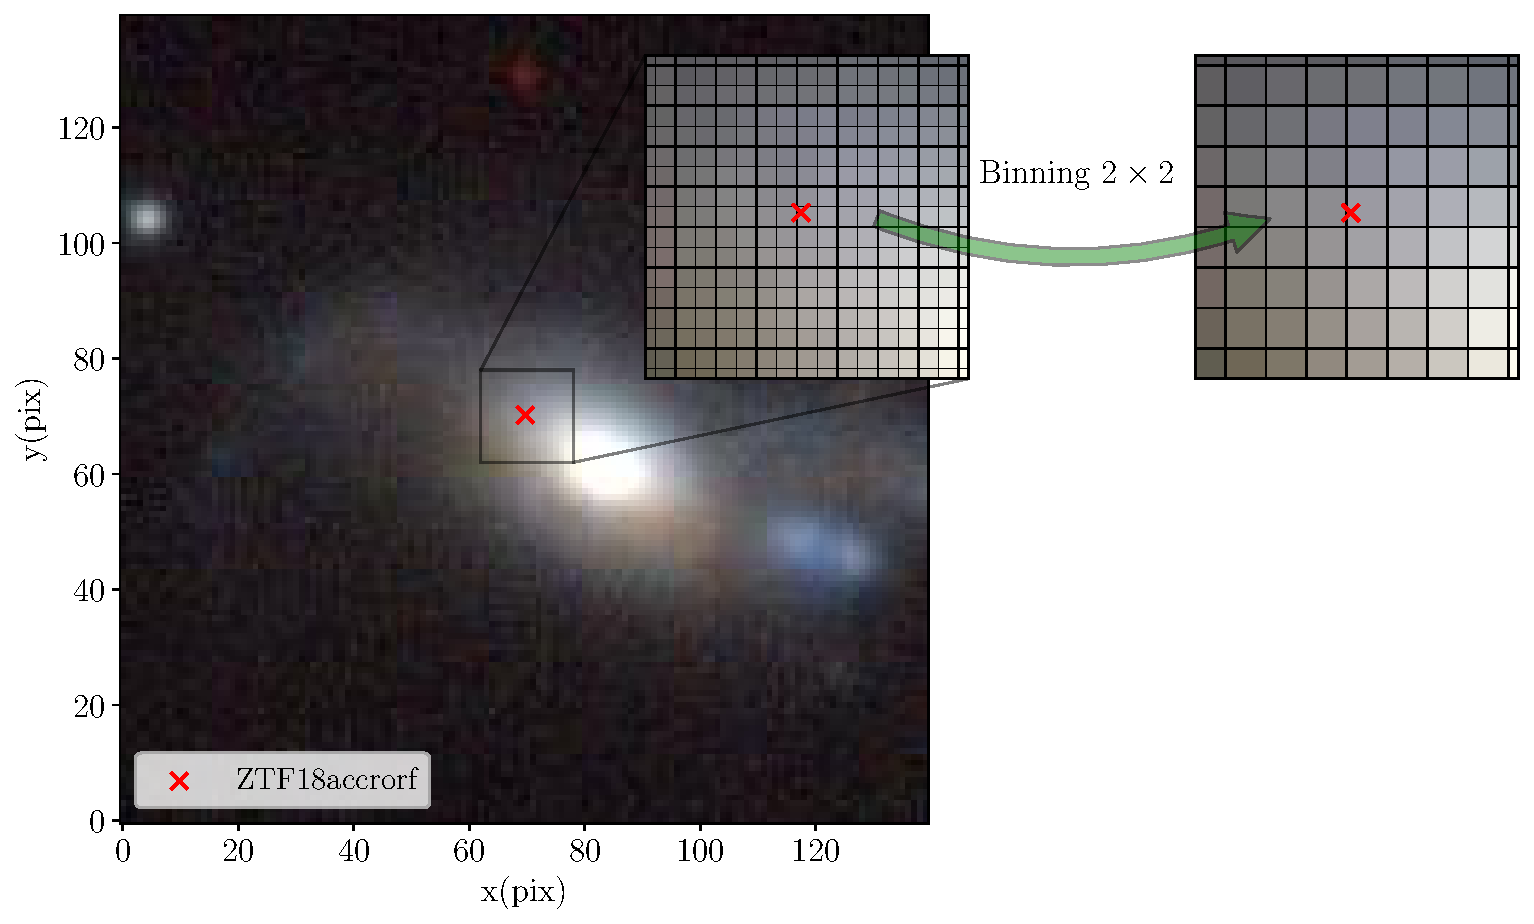
\includegraphics[width=0.99\textwidth]{../figures/05_sedfit/ps_cutouts_ZTF18accrorf_binned.pdf}
  \caption[Illustration binning $2\times2$ sur les images
  PS1.]{Illustration du binning $2\times2$ sur l'image de la Figure~\ref{fig:pscutoutsZTF18accrorf}}
  \label{fig:pscutoutsZTF18accrorf_binned}
\end{figure}

Par ailleurs, le flux (et l'erreur associée) des images étant en unité
de coups, il faut les convertir en unité physique. Nous savons de
\citet{Tonry2012} que le point zéro de
toutes les bandes est de $\SI{25}{mag}$ dans le système de magnitude AB.
En utilisant la définition de ce système de magnitude (Eq~\ref{eq:abmag}), nous
convertissant les unités de flux en mJy, unité physique dans laquelle
les flux doivent être données en entrée de \pkg{CIGALE}. Les
transmissions des bandes photométriques sont également fournies au SED
Fitter, qui les utilise pour intégrer les modèles construits dans les
filtres correspondants et pouvoir ensuite les comparer aux données d'entrée.

\begin{comment}
requiert un flux en unité de mJy,, et que
$f_{\nu}=\frac{\lambda^{2}}{c}f_{\lambda}}$ nous pouvons aisément passer des
unités de coups en unité de flux physique avec un facteur multiplicatif:

\begin{align*}
   f_{\nu}[\erg\ \text{s}^{-1}\cm^{-2}\Hz^{-1}]&=
                                                     10^{-(m_{AB}+48.6)/2.5}\\
  \iff f_{\lambda}[\erg\ \text{s}^{-1}\cm^{-2}\ \text{\AA}^{-1}]&=
                                                                  10^{-(m_{AB}+48.6)/2.5}\frac{c}{\lambda^{2}}\\
  \implies \int f_{\lambda}[\erg\ \text{s}^{-1}\cm^{-2}\
  \text{\AA}^{-1}]\d\lambda&=N_{c}\times 10^{-(m_{AB,0}+48.6)/2.5}\frac{c}{\lambda^{2}}
\end{align*}
avec $N_{c}$ le flux en unité de coups, $\lambda$ la longueur d'onde
pivot de la bande utilisée et $m_{AB,0}$ le point zéro commun aux 5
bandes de PS1. \pkg{CIGALE} requiert un flux en unité de mJy, avec
$1\text{Jy} = 10^{-23}\erg.\sec^{-1}\cm^{-2}\Hz^{-1}$, nous
convertissons donc les flux dans cette unité.
\end{comment}

Par ailleurs, afin d'éviter d'appliquer le SED Fitter sur une zone sans
galaxie (aka fond du ciel), nous effectuons une coupure dans les pixels
où la SED sera modélisée en ne considérant que ceux où le rapport signal
sur bruit (SNR) est supérieur à $3$ dans les $5$ bandes. Une
illustration de cette coupure est montrée dans la Figure~\ref{fig:pscutoutsZTF18accrorf_cutsnr}. 

\begin{figure}[ht]
  \begin{minipage}[c]{0.45\textwidth}
    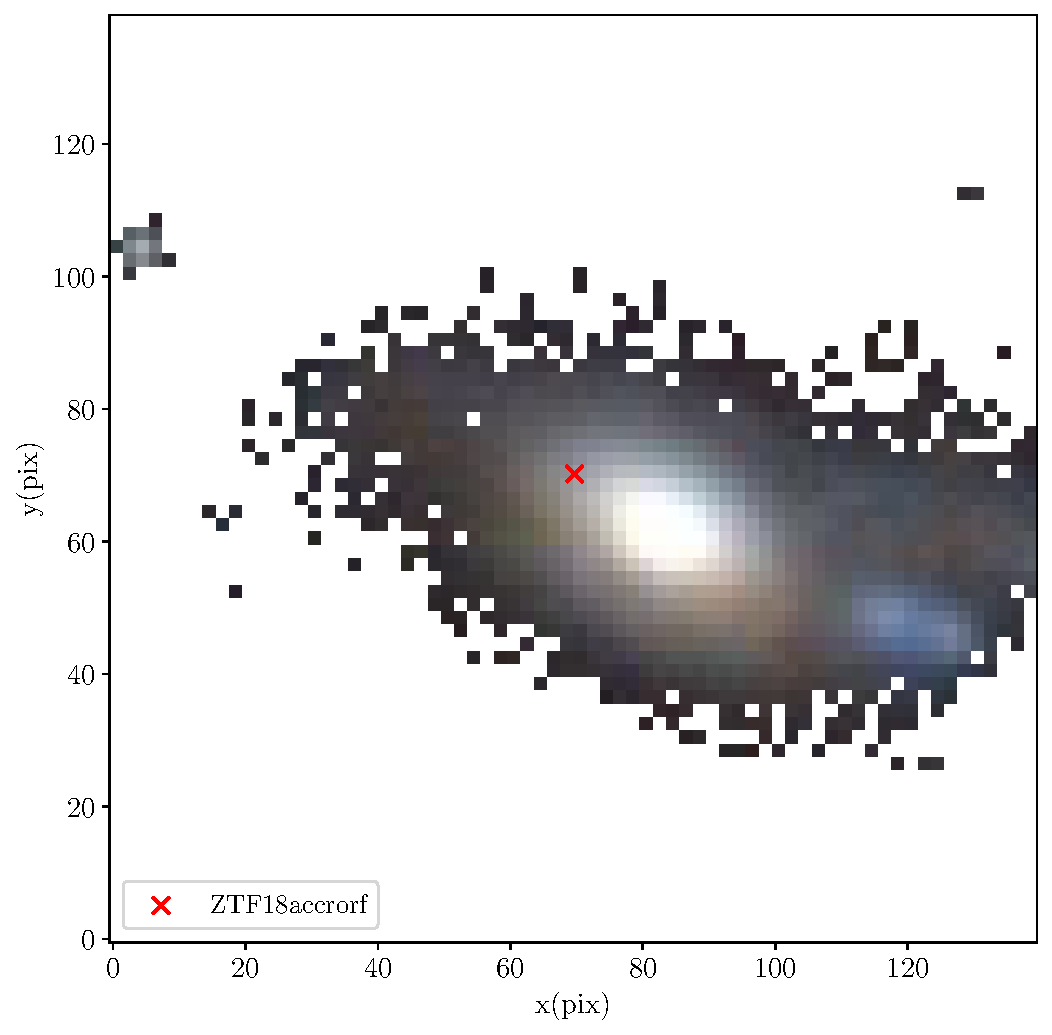
\includegraphics[width=\textwidth]{../figures/05_sedfit/ps_cutouts_ZTF18accrorf_snrcut.pdf}
  \end{minipage}\hfill
  \begin{minipage}[c]{0.53\textwidth}
    \caption[Image RGB de PS1 avec coupure SNR]{Illustration de la
      coupure SNR~$>3$ dans toutes les bandes PS1 avec l'image de la
      Figure~\ref{fig:pscutoutsZTF18accrorf}, après binning $2\times2$.}\label{fig:pscutoutsZTF18accrorf_cutsnr}
  \end{minipage}
\end{figure}

Enfin, à partir des informations de chaque image (flux et
erreurs) nous créons un tableau que \pkg{CIGALE} pourra lire. Ce
dernier contient une colonne \textit{ID}, une colonne \textit{redshift}
(identique pour tous les pixels car nous considérons qu'ils appartiennent au même objet),
et une colonne pour chaque filtre et erreur associée (par exemple
\textit{ps1\_g} et \textit{ps1\_g\_err} pour le flux d'un pixel dans la bande
$g_{P1}$ et l'erreur associée). Le redshift que nous utilisons pour les
galaxies hôtes dans ZTF est habituellement obtenue à
partir de la base de données spectrales de SDSS. Si aucun redshift spectroscopique
n'est disponible, nous utilisons un redshift photométrique, ou un
resdshift spectrale obtenu à partir d'une première extraction de spectre
de la supernova étudiée (voir section~\ref{sec:sniaztf}).

\begin{comment}
Nous montrons un exemple de tableau
d'entrée qui sera lu par \pkg{CIGALE} dans la
Table~\ref{tab:cigaleinput}.

\begin{table}[ht]
    \centerfloat
    \begin{threeparttable}
        \caption{Exemple de tableau d'entrée pour \pkg{CIGALE}}
        \label{tab:cigaleinput}
        
        \begin{tabular}{lcccccccc}
        \toprule
           id &  redshift &     ps1\_g &  ps1\_g\_err &     ps1\_r &  ps1\_r\_err &   \ldots   &     ps1\_y &  ps1\_y\_err \\
        \midrule
           52 &      0.042 &  0.000698 &   0.000052 &  0.001043 &   0.000070 & \ldots &  0.001230 &   0.000373 \\
          120 &      0.042 &  0.000586 &   0.000051 &  0.000901 &   0.000068 &  \ldots &  0.001214 &   0.000346 \\
          121 &      0.042 &  0.001735 &   0.000058 &  0.002405 &   0.000072 &  \ldots &  0.002118 &   0.000350 \\
          122 &      0.042 &  0.001982 &   0.000059 &  0.003414 &   0.000075 & \ldots &  0.003940 &   0.000389 \\
          123 &      0.042 &  0.001114 &   0.000055 &  0.001932 &   0.000071 &  \ldots &  0.001633 &   0.000398 \\
          \vdots & \vdots &\vdots &\vdots &\vdots &\vdots &\vdots &\vdots &\vdots \\
          \bottomrule
        \end{tabular}
        \begin{tablenotes}[flushleft]
        \item \textbf{Notes.} Chaque ligne (id) correspond à un pixel. Le redshift est le même pour tous les
          pixels car on considère qu'ils appartiennent tous au même
          objet. L'Unité des flux est en mJy.
        \end{tablenotes}
    \end{threeparttable}
  \end{table}
\end{comment}
La géométrie et la position spaciale de chaque pixels sont alors mis en
mémoire vis à vis de leur identifiant, et les pixels non sélectionnés
par la coupure en SNR se verront attribués un spectre nul lors de la construction du cube intrinsèque.

\subsection{Configuration de \pkg{CIGALE}}
\label{ssec:cigaleconfig}

Nous utilisons dans le pipeline \hypergal\ la version 2020 de
\cigale. Trois étapes sont nécessaires pour faire tourner le code :
l'initialisation, la génération du fichier de configuration et enfin le
lancement de l'ajustement. Ces étapes nécessitent la modification manuelle de
fichiers \textit{.ini}, nous avons donc créé dans \hypergal\ une méthode d'automatisation de ces processus.

L'initialisation a pour but de fixer le fichier de données à utiliser, le nombre de coeur sur la machine à
utiliser et surtout les modules à partir desquels la grille de modèles
sera calculée. Détaillons à présent les différentes composantes qui constitueront les ingrédients de notre modéliseur de SED.

\subsubsection{Histoire de formation stellaire}

Le premier module va définir le modèle d'histoire de formation stellaire
(SFH) et ainsi le taux de formation stellaire (SFR) au cours du
temps. La SFH décrit le processus de formation des étoiles au sein de la
galaxie, qui va dépendre du temps et de l'espace, et peut se produire de
façon brutale (\textit{burst}), progressive, voire les deux
combinés. Nous avons choisi d'utiliser le module
\textbf{\pkg{sfhdelayed}} proposé par \cigale, où la modélisation est de la forme suivante:
\begin{equation}
  \label{eq:sfhdelayed}
  SFR_{delayed}(t)\propto \frac{t}{\tau^2}\times\exp(-t/\tau) \text{ pour $0\le t\le t_0$}
\end{equation}
avec $t_0$ l'âge de commencement de la formation stellaire, et $\tau$ le
temps caractéristique. Cette forme permet une évolution lisse dans le
temps, avec une croissance quasi-linéaire de la SFR jusqu'à un pic de
taux de formation, suivant d'une lente décroissance quand $t>\tau$.
Pour plus de flexibilité et prendre en compte un possible épisode de
formation stellaire tardif, ce module permet également de rajouter une
seconde composante exponentielle \citep{Malek2018}.
Ainsi, la forme fonctionnelle de la SFR est:
\begin{equation}
  \label{eq:sfhdelayedburst}
  SFR(t) = SFR_{delayed}(t) + SFR_{late}(t)
\end{equation}
où $SFR_{delayed}(t)$ est la composante de
l'équation~\ref{eq:sfhdelayed}, et $SFR_{late}(t)\propto
e^{(-(t-t_{late})/\tau_{late})}$ quand $t>t_{late}$, $0$
sinon. L'amplitude de cet épisode tardif est fixée par le paramètre
$f_{late}$, qui est défini comme le ratio entre la masse d'étoiles
formées durant cet évènement et la masse totale d'étoiles. Les
paramètres utilisés ($\tau$, $\tau_{late}$, $t_0$, $t_{late}$ et
$f_{late}$) sont présentés dans la Table~\ref{tab:cigaleparams}.

\subsubsection{Population stellaire}
Le second module décrit la population stellaire à laquelle la SFH va
être appliquée, ce qui va permettre le calcul de la composante stellaire
du spectre de la SED. Nous utilisons dans \hypergal\ la librairie de
populations stellaires simple \textbf{\pkg{bco3}} (ou \pkg{GALAXEV}) de
\citet{BCO3}, avec la fonction initiale de masse de
\citet{Chabrier2003}. Cette librairie de population est disponible avec
un large intervalle de paramètres de metallicité $Z$\footnote{Définie comme
  la fraction massique des éléments plus lourd que l'hélium, vérifiant
  la relation $X+Y+Z=1$ où $X$ et $Y$ représentent les fractions massiques
  de l'hydrogène et l'hélium respectivement.}, allant de $0.0001$ à
$0.05$, et fournit une résolution de l'ordre de $3$\AA\ sur l'intervalle
de longueur d'onde $[3200-9500]$\AA\ (et une plus faible résolution au delà).


\subsubsection{\'Emission nébulaire}

Une part importante de lumière émise par les étoiles les plus massives
(dans le continuum Lyman) a pour effet de ioniser le gaz présent au sein
de la galaxie. Ce phénomène engendre à son tour une émission énergétique
non négligeable sous la forme de continuum et de raies. La librairie
utilisée par \cigale\ pour modéliser l'émission nébulaire est basée sur
\citet{Inoue2011}, et généré avec \pkg{CLOUDY 13.01} \citep{Ferland2013}.
La modélisation qui en découle fixe les intensités relatives de 124
raies d'émissions dans la région $HII$, et est paramétrisée par la
métallicité $Z$ (identique à celui utilisé pour la population stellaire)
et un paramètre d'ionisation $U$ sans dimension. Ce paramètre est défini
tel que $\log(U)\equiv \log(n_{\gamma}/n_H)$ où $n_{\gamma}$ est la
densité numérique de photons responsables de l'ionisation d'hydrogène et
$n_H$ la densité numérique d'hydrogène.

L'émission nébulaire ayant une forte contribution dans l'optique, nous
explorons une large gamme de paramètres de métallicités $Z$ et de
paramètres d'ionisation $U$, décrite dans la Table~\ref{tab:cigaleparams}.

\subsubsection{Loi d'atténuation}

La poussière contenue dans la galaxie absorbe fortement les radiations à
courte longueur d'onde, notamment de l'ultraviolet au proche infrarouge,
et cette énergie est ensuite ré-émise dans l'infrarouge moyen et
lointain. Considérant le fait que \hypergal\ est conçu pour des objets
jusqu'à un redshift de $z\approx0.1-0.15$, et que nous utilisons des
images photométriques entre environ $4000$ et $10000$\AA, l'effet de
l'atténuation par la poussière ne doit surtout pas être négligé.

Nous adoptons le modèle développé par \citet{CharlotFall2000}, à travers
le module \textbf{\pkg{dustatt\_modified\_CF00}} (CF00) de
\cigale. L'idée de ce modèle est de considérer 2 populations d'étoiles:
les étoiles jeunes ($<10^7$ années) qui résident encore dans le nuage
qui leur a donné naissance (\textit{birth cloud}; BC), et les étoiles
vieilles ($>10^7$ années) qui elles sont considérées comme appartenant
au milieu interstellaire (ISM). L'atténuation est donc traitée
différemment, dans le premier cas la contribution du nuage et du milieu
interstellaire sont pris en compte, dans le second cas seul le milieu
interstellaire. Une loi de puissance est utilisée dans les 2 cas,
normalisée par l'atténuation dans la bande V ($\lambda_V=\SI{0.5}{\micro\metre}$):

\begin{align*}
  A_{\lambda}^{BC}=&A_{V}^{BC}\left(\frac{\lambda}{\lambda_V}\right)^{n_{BC}}\\
  A_{\lambda}^{ISM}=&A_{V}^{ISM}\left(\frac{\lambda}{\lambda_V}\right)^{n_{ISM}}
\end{align*}
et le rapport entre l'atténuation dans la bande V des étoiles jeunes et des étoiles vieilles est paramétré par:

\begin{equation*}
  \mu=\frac{A_{V}^{ISM}}{A_{V}^{ISM}+A_{V}^{BC}}
\end{equation*}
où $\mu$ est un paramètre libre pour plus de fléxibilité et une
meilleure estimation des raies d'émission $\text{H}_{\alpha}$
\citep{Battisti2016,Buat2018,Malek2018,Chevallard2019}.
Nous choisissons de fixer la pente de la loi de puissance pour
l'atténuation du milieu interstellaire à $n_{ISM}=-0.7$ en suivant
\citet{CharlotFall2000}. Cependant nous fixons l'autre pente
(contribution du nuage) à $n_{BC}=-1.3$ pour prendre en compte les
effets d'absorption des grains dans l'optique similairement à ceux
présents dans la Voie Lactée et les nuages de Magellan \citep{LoFaro2017,Wild2007,Cunha2008MAGPHYS,Battisti2019}.

\subsubsection{\'Emission de la poussière}

La poussière ré-émet l'énergie absorbée entre l'UV et le proche IR dans
le moyen et lointain IR. \'Etant donné que l'on étudie des galaxies
proches ($z<0.15$) avec des bandes photométriques définies sur un
interval de longueur d'onde
${\lambda\lesssim10000}$ \AA, cette contribution n'a pas d'impact
dans notre cas d'utilisation. En testant plusieurs modèles et
différentes libertés, nous n'avons observé aucun changement dans le modèle ajusté. Nous utilisons donc par défaut le module le plus
simple décrivant cette contribution, \textbf{\pkg{dale2014}}
\citep{Dale2014}. La paramétrisation est de la forme ${\d M_{\d}(U)\propto
U^{-\alpha}\d U}$, entièrement défini par l'exposant $\alpha$, avec
$M_{\d}$ la masse de poussière chauffée par le champ radiatif et $U$ l'intensité énergétique d'exposition.


\begin{table}[h]
  \scriptsize
  \centerfloat
  \setlength\tabcolsep{14pt}
  \renewcommand{\arraystretch}{1.5}
    %\begin{threeparttable}
        \caption{Paramètres d'entrées  pour chaque module de \cigale
          utilisé.}
        \label{tab:cigaleparams}
        \makebox[\textwidth]{\begin{tabularx}{1.2\textwidth}{ccc}
                               \toprule                               
                               \textbf{Paramètre} & \textbf{Symbole} &
                                                                       \textbf{Valeurs
                                                                       de
                                                                       liberté}\\            
                               \midrule
                                                   & \textbf{Histoire de
                                                     formation stellaire
                                                     (SFH)} & \\
                               \hline 
          \textit{e-folding time} population stellaire principale &
                                                                    $\tau_{main}$(Myr)& $1000$, $3000$, $5000$\\
                               
          \textit{e-folding time} population stellaire tardive &
                                                                 $\tau_{late}$(Myr)& $10000$\\
                               
          Âge population stellaire principale & $age_{main}$(Myr)&
                                                                   $1000$, $2000$, $4000$, $8000$, $10000$, $12000$\\
                               
                               Âge population stellaire tardive & $age_{late}$(Myr)& $10$, $40$, $70$\\
                               
          Fraction massique de la population tardive & $f_{late}$ &
                                                                      $0$, $0.001$, $0.01$, $0.1$, $0.2$\\
                               
                               \hline
                               
                                                   & \textbf{Population stellaire} & \\
                               \multicolumn{3}{c}{Modèles de population stellaire
                                 \citet{BCO3}}\hspace{-1.1cm}\\
                               
                               
                               \hline
                               Fonction initiale de masse & IMF & \citet{Chabrier2003}\\
                               
          Metallicité & $Z$ & $0.0001$, $0.0004$, $0.004$, $0.008$,
                              $0.02$, $0.05$\\
                               
                               \hline                               

                                                   & \textbf{\'Emission
                                                     nébulaire} & \\
                               \hline
                               
                               Paramètre d'ionisation& $\log(U)$& $-4$, $-3$, $-2$, $-1$\\
                               
                               \hline
                                                   & \textbf{Atténuation
                                                     de la
                                                     poussière}&\\
                               \multicolumn{3}{c}{Basé sur
                               \citet{CharlotFall2000} et \citet{Buat2018}}\hspace{-1.1cm}\\
                               \hline
                               Atténuation milieu interstaire dans la
                               bande V & $A_{V}^{ISM}$&$0$, $0.3$,
                                                        $0.7$, $1$,
                                                        $1.3$, $1.7$,
                                                        $2$\\
                              
                               $\frac{A_{V}^{ISM}}{A_{V}^{ISM}+A_{V}^{BC}}$
                                                   & $\mu$ & $0.1$,
                                                             $0.3$,
                                                             $0.7$,
                                                             $1$\\
                               Pente loi de puissance BC & $n_{BC}$&
                                                                     $-1.3$\\
                               Pente loi de puissance ISM & $n_{ISM}$& $-0.7$\\
                               \hline
                                                   & \textbf{\'Emission
                                                     de la
                                                     poussière}&\\
                               \multicolumn{3}{c}{Librairie de \citet{Dale2014}}\hspace{-1.1cm}\\
                               \hline
                               Exposant $\alpha$ & $\alpha$ & $1$\\

                               \bottomrule
        \end{tabularx}}
        \begin{tablenotes}[flushleft]
        \item \textbf{Notes.} Chaque \textit{e-folding time} correspond au
          temps caractéristique des 2 exponentielles décroissantes de
          l'équation~\ref{eq:sfhdelayedburst}. 
        \end{tablenotes}
      %\end{threeparttable}
      
    \end{table}
    
\subsection{Utilisation}
    
La configuration que nous proposons dans la Table~\ref{tab:cigaleparams}
nécessite le calcul d'une grille de $181440$ modèles. Sachant que notre
but n'est pas de dériver de paramètres physiques (voir
\citet{Boquien2019} pour la liste exhaustive), mais de seulement modéliser le
SED pour chaque pixel spectral, nous
gagnons un temps de calcul non négligeable. 
Avec une machine de $20$ coeur, l'ajustement des SED de chaque pixel prend environ $3$ minutes.

Avant de construire le cube intrinsèque, nous récupérons l'information
spatiale propre à chaque pixel, devenu nos nouveaux spaxels du cube intrinsèque, afin de
réaranger le même agencement que l'image dans la
Figure~\ref{fig:pscutoutsZTF18accrorf_cutsnr}.

La Figure~\ref{fig:cigalesinglespectra} montre deux exemples de SED
ajustées par \cigale, l'un à l'intérieur du bulbe galactique, l'autre à l'extérieur.

\begin{figure}[ht]
  \centering
  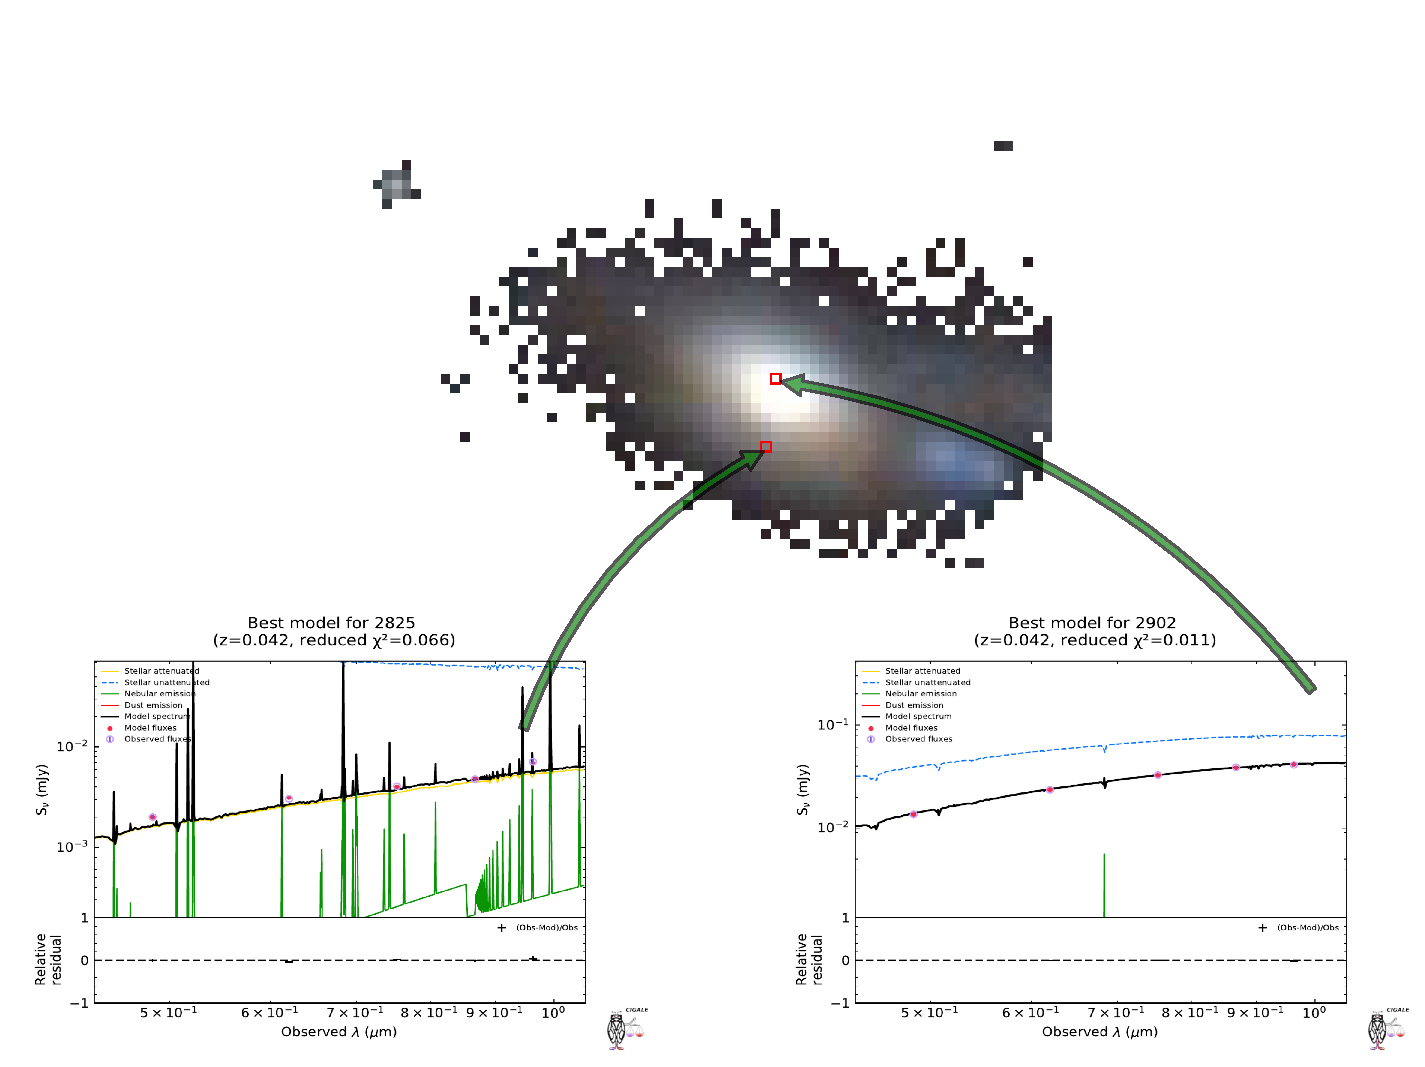
\includegraphics[width=0.99\textwidth]{../figures/05_sedfit/cigalesinglespectra.pdf}
  \caption[Exemples de SED fittés]{Exemples de SED ajustées pour deux
    pixels. \textit{À gauche} un pixel à l'extérieur du bulbe de la
    galaxie, \textit{à droite} un pixel à l'intérieur. Les différentes
    composantes de la SED totale sont indiqués dans les figures de
    sortie de \cigale.}
  \label{fig:cigalesinglespectra}
\end{figure}

L'obtention de la SED permet également de déterminer le flux intégré spectralement sur
les bandes photométriques d'entrée, et ainsi d'estimer la qualité de
la modélisation et la présence éventuelle de structures dans les résidus. Nous montrons par exemple dans la
Figure~\ref{fig:cigale_pullrms} la distribution du pull vis à vis de
chaque bande de PS1, ainsi que le RMSE spectral en les considérant
toutes.

Le pull est défini comme la déviation entre le modèle et les données,
pondérée par l'erreur sur ces dernières, tel que:
\begin{equation}
  \label{eq:pull}
  p = \frac{y - \widetilde{y}}{\sigma}
\end{equation}
avec $\widetilde{y}$ la prédiction du modèle, $y$ la donnée et $\sigma$
l'erreur sur $y$.
Le RMSE (ou erreur quadratique moyenne), est défini tel que:

\begin{equation}
  \label{eq:rms}
  RMSE = \sqrt{\left(\frac{1}{N_{\lambda}}\sum_{\lambda}\left(\frac{y_{\lambda} - \widetilde{y}_{\lambda}}{y_{\lambda}}\right)^{2} \right)}
\end{equation}
avec la même définition des paramètres que pour le pull et $N_{\lambda}$
étant le nombre de données spectrales ($5$ dans notre cas). On notera la
normalisation par $y_{\lambda}$, afin d'avoir une quantité plus
facilement interprétable.

\begin{figure}[ht]
  \centering
  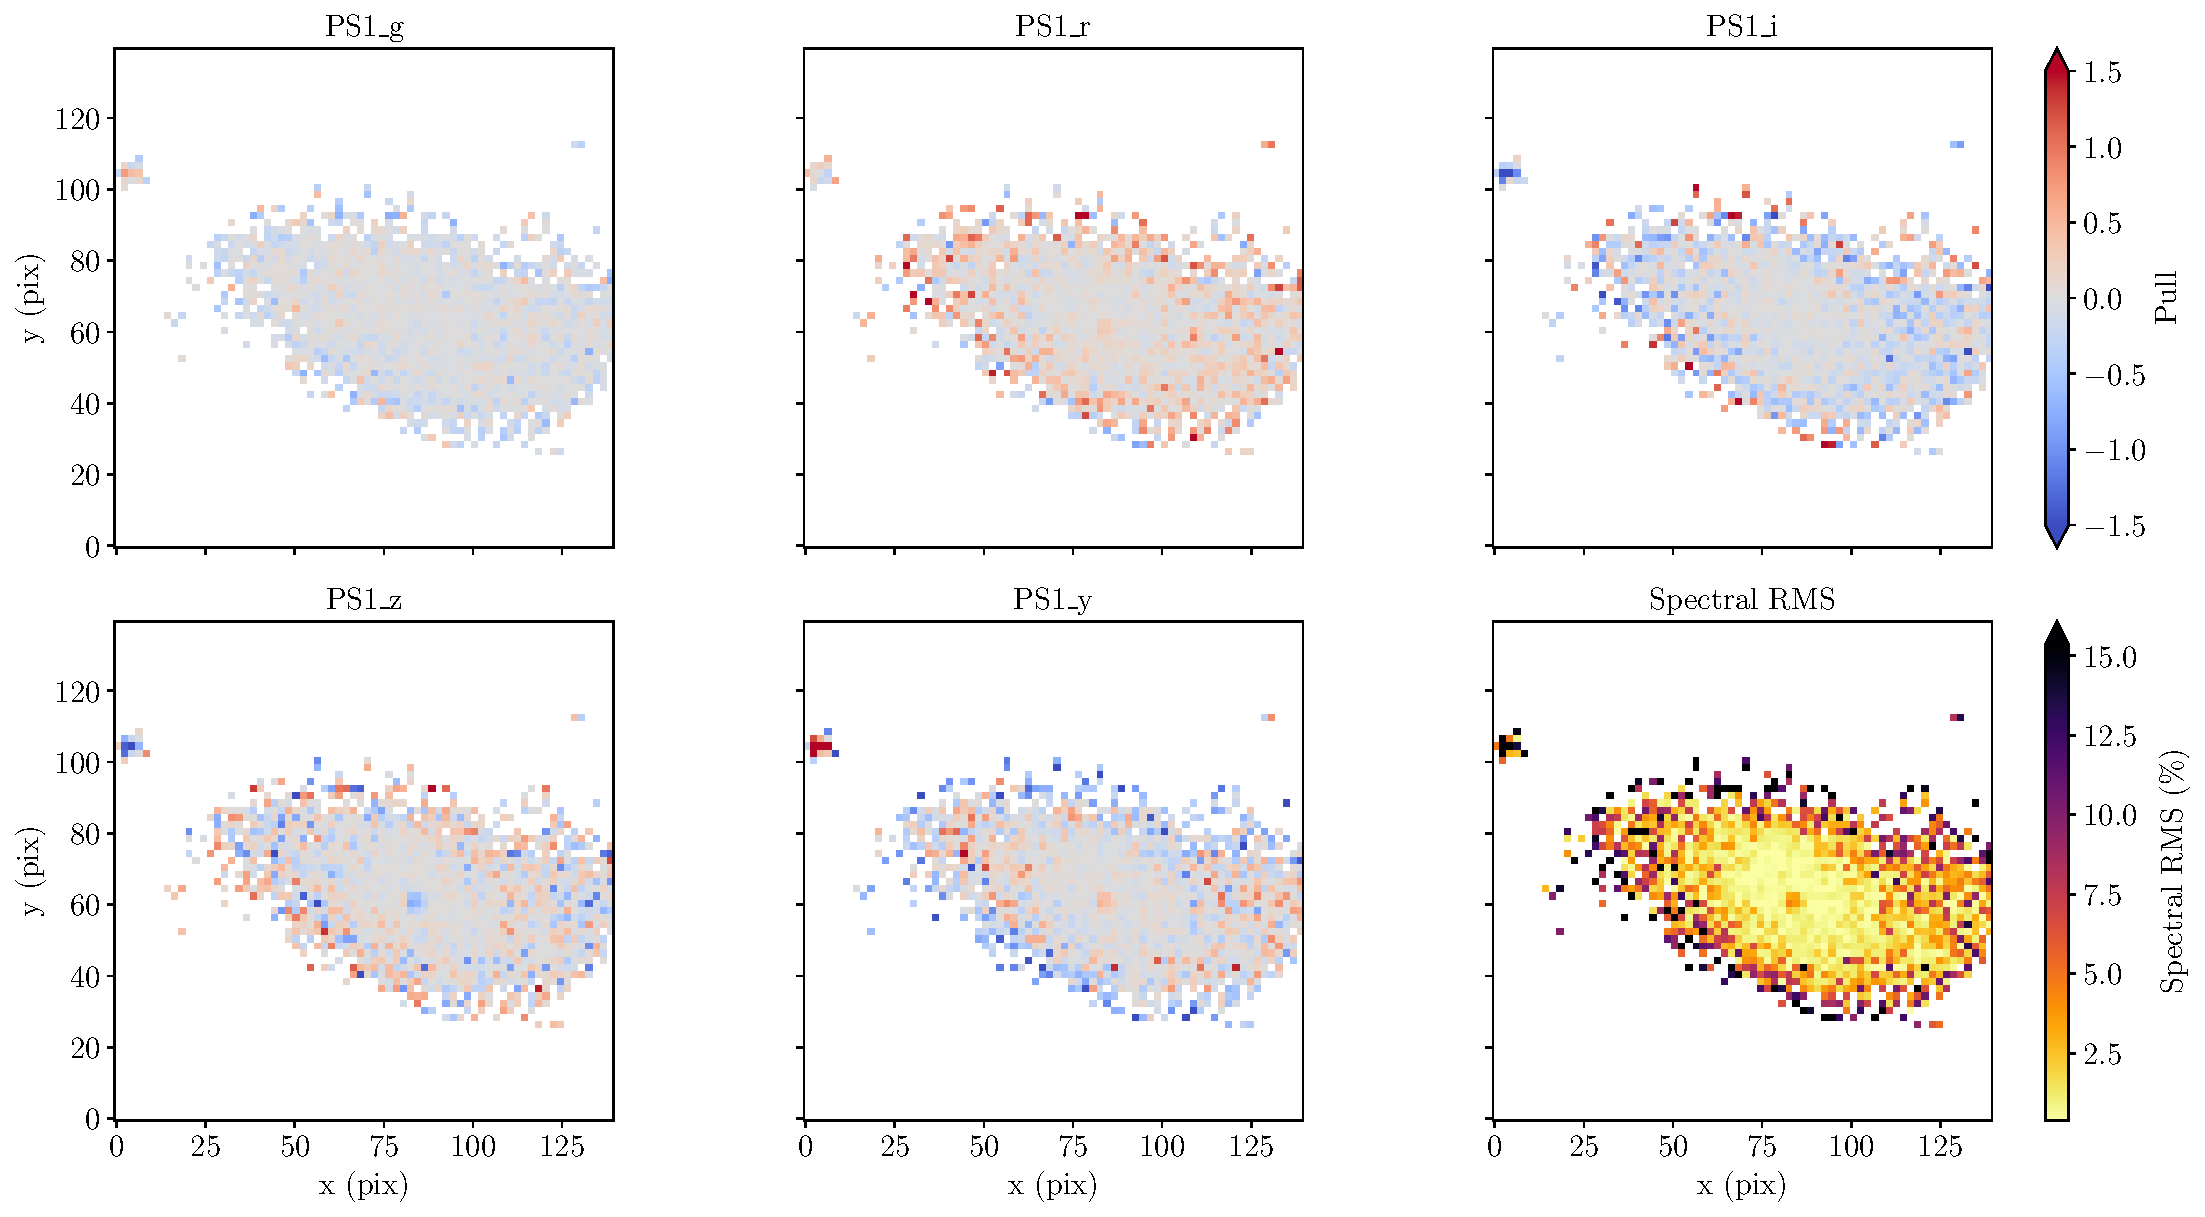
\includegraphics[width=0.99\textwidth]{../figures/05_sedfit/cigale_pullrms_ZTF18accrorf.pdf}
  \caption[Cartographie du pull et du RMS en sortie de
  \cigale]{Cartographie du pull pour chaque bande PS1 et du RMS spectral en sortie de \cigale}
  \label{fig:cigale_pullrms}
\end{figure}

Nous obtenons dans ce cas de figure une distribution sans structure
apparente du pull et du RMS, avec une précision de l'ordre de $2-3$\%
dans une majorité de la galaxie. On notera une déviation non néglieable
sur les bords de la galaxie où la coupure $\text{SNR}>3$ n'est peut-être pas
assez stricte et laisse passer quelques zones du ciel non modélisables
par le SED Fitter.

Nous pouvons estimer le RMS spatial global à partir du RMS spectral de
chaque pixel, tel que:
\begin{equation}
\text{RMS}_{spatial} =\sqrt{\left(\frac{1}{N_{p}}\sum\limits_{p} \left(\text{RMS}^{2}_{p}\right)\right)}
\end{equation}

En considérant les $90$ premiers percentiles en RMS des pixels, nous obtenons avec les résultats montrés dans la
Figure~\ref{fig:cigale_pullrms} que le $\text{RMS}_{spatial}=2.9\%$.
\clearpage
\section{Construction du cube intrinsèque}\label{sec:intcube}

\subsection{\'Echantillonnage des spectres dans l'espace SEDm}
% \label{ssec:xxx}

Chaque pixel étant traité indépendamment par \cigale, leur échantillonnage
spectral de sortie n'est pas homogène, et nécessite donc d'être uniformisé à
notre cas d'utilisation, à savoir l'échantillonnage spectral de la SEDm.

Les cubes de la SEDm sont construits numériquement avec les modules
\pkg{pyifu}\footnote{\url{https://github.com/MickaelRigault/pyifu}} et
\pkg{pysedm}, écrits en \pkg{python}, et sont composés de $220$ tranches spectrales
étendues de $3700$\AA\ à $9300$\AA\, soit un échantillonnage spectral
d'environ $25.57$\AA.

Nous illustrons dans la Figure~\ref{fig:cigalesampling}
l'échantillonnage spectral d'une SED obtenue avec \cigale, et sa
projection dans l'espace spectral de la SEDm.
Initialement, l'échantillonnage est inférieur à
$5$ \AA, mais n'est pas uniforme. Pour effectuer le ré-échantillonnage
correspondant à l'espace spectral de la SEDm, nous interpolons par une
spline cubique la SED obtenue avec \pkg{Cigale}, avec un échantillonnage $10$
fois plus fin (2200 pixels).
Nous prenons en compte de cette façon le fait que chaque valeur de flux correspond à un
flux intégré, et non discret. 
Nous appliquons ensuite une convolution par une fonction porte (de
taille $10$ pixels également) pour
obtenir notre spectre échantillonné dans l'espace spectral de la SEDm (220 pixels
spectraux entre $3700$\AA\ et $9300$\AA\ ) .

\begin{figure}[ht]
  \centering
  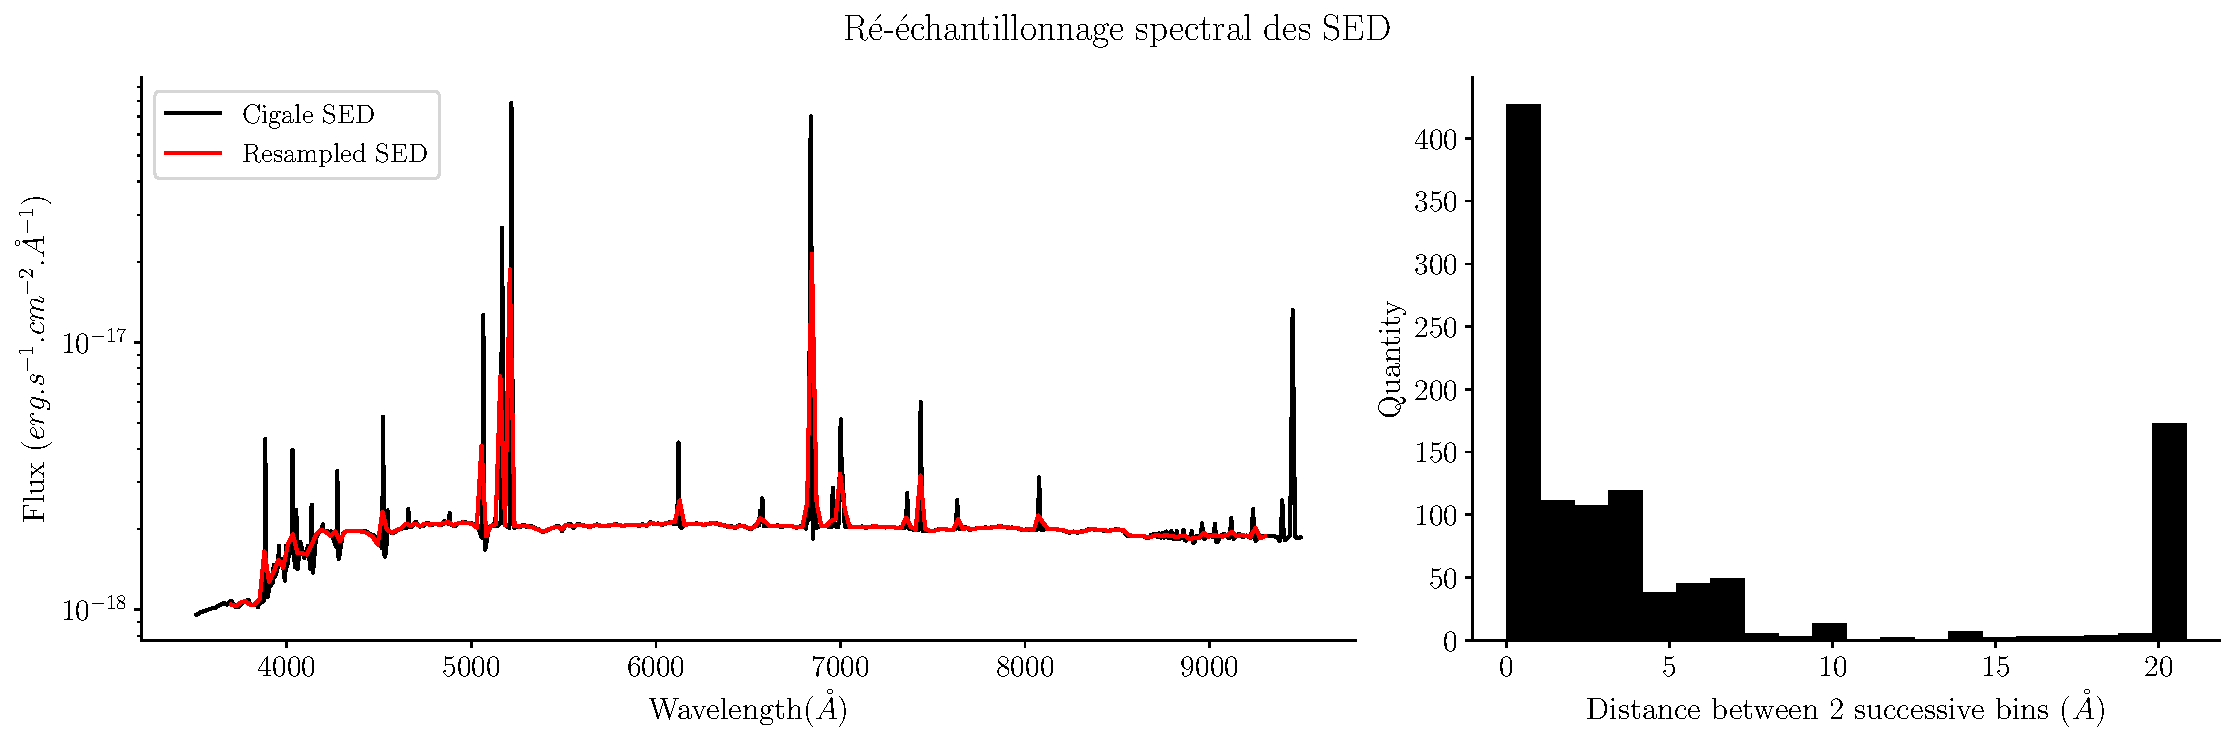
\includegraphics[width=0.98\textwidth]{../figures/05_sedfit/cigalesampling.pdf}
  \caption[\'Echantillonnage spectral d'une SED obtenue avec
  \cigale]{\'Echantillonnage spectral d'une SED obtenue avec \cigale. \textit{À
    gauche} la SED de sortie de \cigale entre $3500$ et $9500$\AA\ 
    (courbe noir) et le ré-échantillonnage dans l'espace spectral de la SEDm
    (courbe rouge). \textit{À droite} nous montrons l'histogramme
    de la taille d'échantillonnage de cette SED à la sortie de \cigale.}\label{fig:cigalesampling}
\end{figure}

\subsection{Construction du cube}
% \label{ssec:xxx}

Ayant projeté toutes les SED dans l'espace spectral de la SEDm,
nous sommes à présent en mesure de reconstruire le cube intrinsèque
de la galaxie hôte.

Nous rappelons que nous avons effectué une coupure $\text{SNR}>3$ (section~\ref{ssec:preprocessimages}) dans toutes
les bandes PS1 pour isoler les zones des images photométriques
n'appartenant pas à une source astronomique. Pour ces zones nous fixons
une SED nulle, le fond ayant déjà été soustrait dans les images
PS1 (section~\ref{ssec:preprocessps1}).

Nous utilisons alors la mise en mémoire de la géométrie et localisation
spatiale de chaque pixel avant l'utilisation de \cigale, pour procéder
à l'agencement de nos spaxels.
Nous montrons dans la Figure~\ref{fig:intcube_ZTF18accrorf} le cube intrinsèque
ainsi reconstruit.

\begin{figure}[ht]
  \centering
  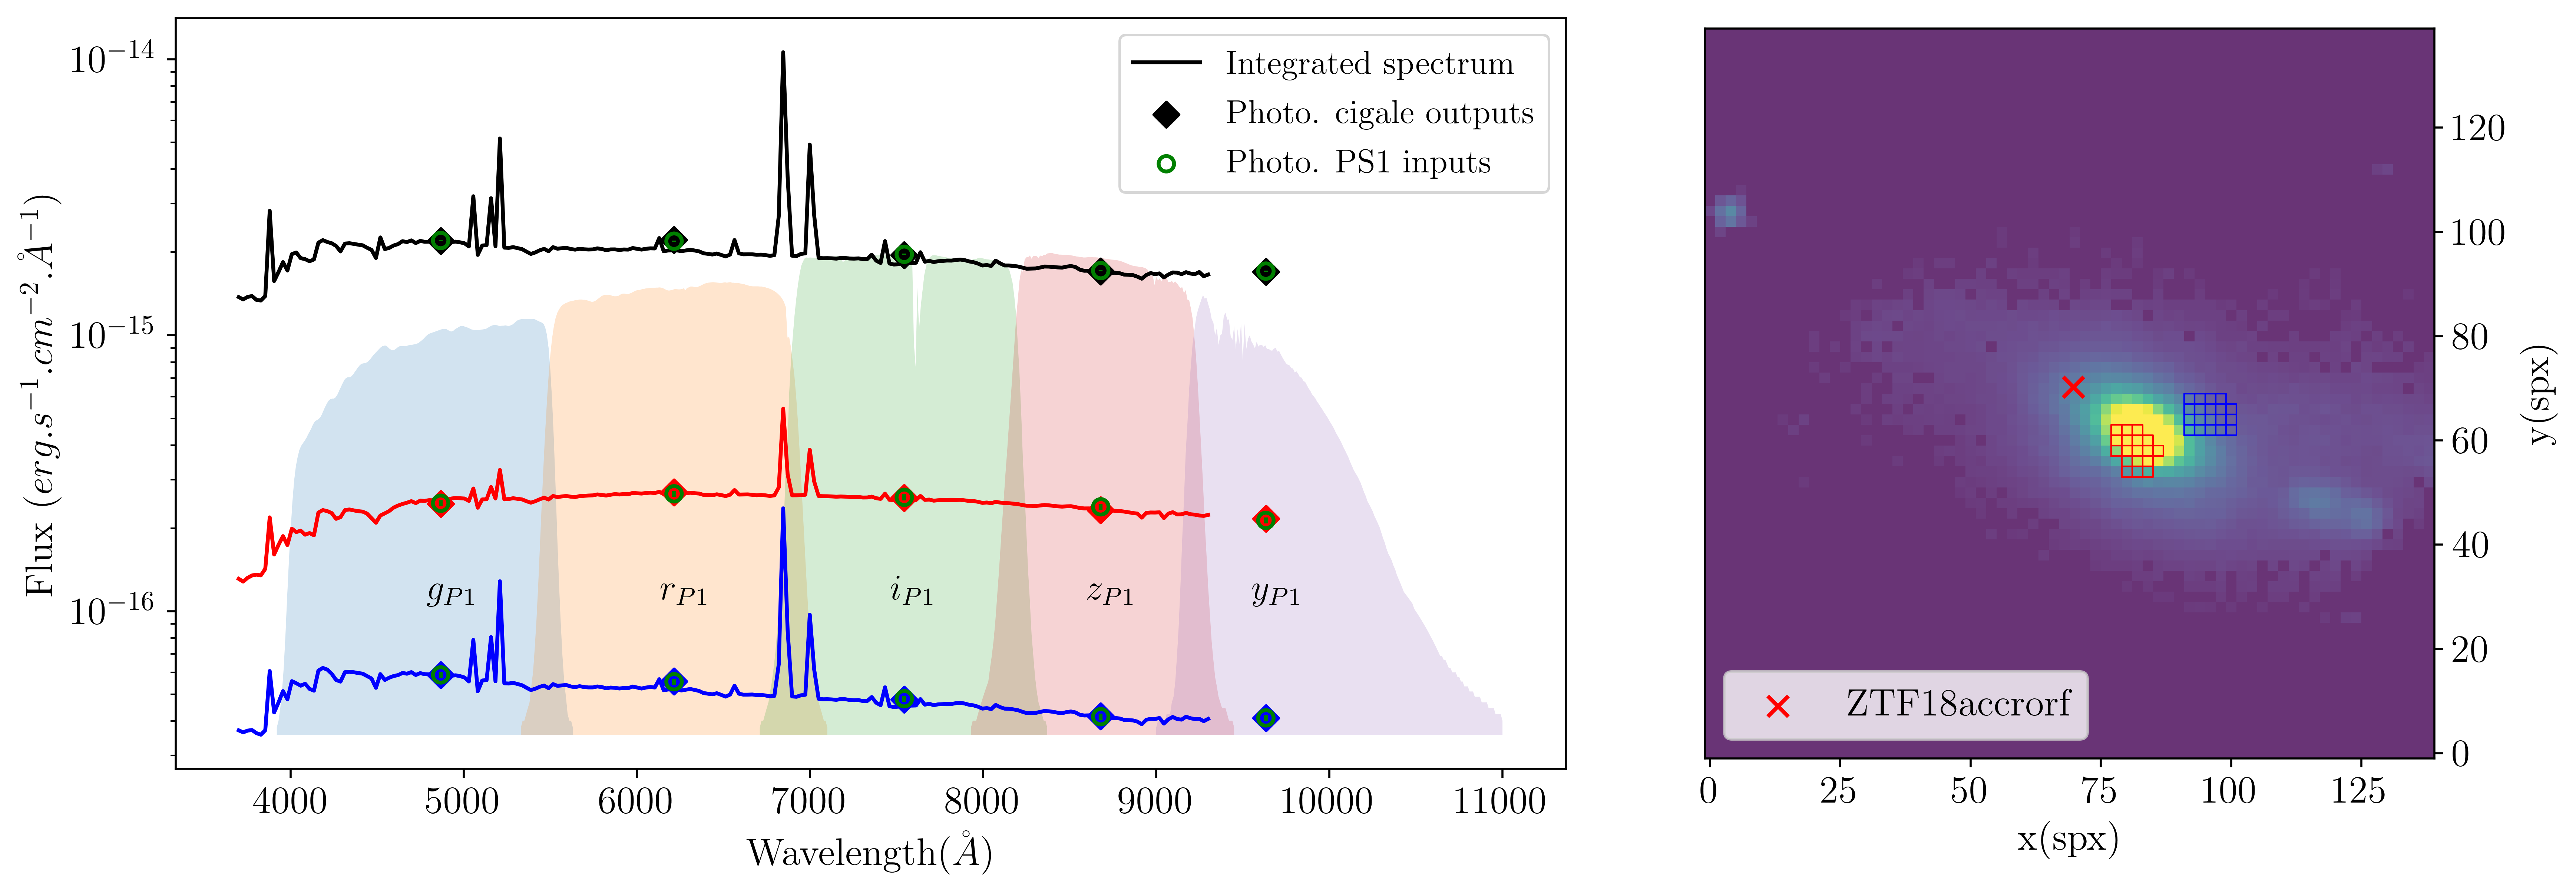
\includegraphics[width=0.97\textwidth]{../figures/05_sedfit/intcube_ZTF18accrorf.png}
  \caption[Cube intrinsèque de la galaxie hôte de ZTF18accrorf]{Cube
    intrinsèque de la galaxie hôte de ZTF18accrorf. \textit{À droite}
    l'image 2D du cube 3D avec toutes les tranches de longueur d'ondes
    empilées. La croix rouge indique la position prédite de
    ZTF18accrorf. Les spaxels sélectionnés en rouge et bleu servent à
    illustrer l'aspect 3D du cube en montrant la SED
    correspondante. \textit{À gauche} sont représentés les spectres intégrés de 3
    différentes zones spatiales du cube. Les spectres bleu et rouge
    correspondent aux spaxels de même couleur, et le spectre noir à
    l'intégration total. La couverture spectrale des filtres de PS1 est
    également représentée, avec pour chaque spectre les données
  photométriques d'entrée (\textit{cercles verts}) et le résultat obtenu avec
  \cigale (\textit{losanges}) à la longueur d'onde pivot du filtre.}\label{fig:intcube_ZTF18accrorf}
\end{figure}


L'obtention du cube intrinsèque clôture l'étape de la modélisation hyperspectrale
d'\hypergal. Le code dédié à la requête des images photométriques PS1 et
leur traitement pour le SED fitting est contenu dans le module
\pkg{hypergal.photometry}. L'utilisation de \cigale est entièrement
automatisée dans le module \pkg{hypergal.spectroscopy.sedfitting}, avec
la liberté laissée à l'utilisateur d'utiliser une configuration
différente de celle implémentée par défaut
(Table~\ref{tab:cigaleparams}) dans un fichier \textit{.json}. Ce
module traite également la reconstruction du cube.

La projection dans l'espace des observations de la SEDm n'est pas encore
possible à ce stade, car nous n'avons pas pris en compte la réponse
impulsionnelle de notre instrument. En effet, les réponses impulsionnelles spectrale
(fonction d'étalement de raie; LSF) et
spatiale (fonction d'étalement de point; PSF) de la SEDm ne sont pas
les mêmes que celles présentes dans notre cube.

Les SED obtenues avec
\cigale sont à la résolution spectrale des modèles de
population stellaire. La librairie \pkg{bc03} que nous avons utilisée
est basée sur des spectres ayant une résolution de $3$\AA\ sur
l'intervalle [$3200$-$9500$]\AA\ (correspondant à une résolution de
$R=\lambda/\d\lambda\approx2000$; \citet{BCO3}). Cette résolution,
$20\times$ supérieur à celle de la SEDm, rend primordiale l'étude la
LSF.

La PSF de notre cube provient quant à elle de nos images
photométriques PS1, qui est chromatique et que nous avons détaillé dans
la Table~\ref{tab:3pisteradian} (un seeing typiquement de l'ordre de
$\sim1\farcs1$ contre $\sim1\farcs7$ pour la SEDm).

Le chapitre suivant de
ce manuscrit a pour but de caractériser ces différentes réponses
instrumentales.

%\bibliographystyle{../main/aa_url2}
%\bibliography{99_references}

\end{document}

%%% Local Variables:
%%% mode: latex
%%% TeX-master: t
%%% End:
